\section{Alarm data transmission: ReMeS}
\label{scenario:remes-alarm}

\npar Figure \ref{fig:scenario-5-10} shows the sequence diagram for the scenario
``Alarm data transmission: ReMeS''.

\begin{figure}[H]
	\begin{centering}
		% TODO Figure
		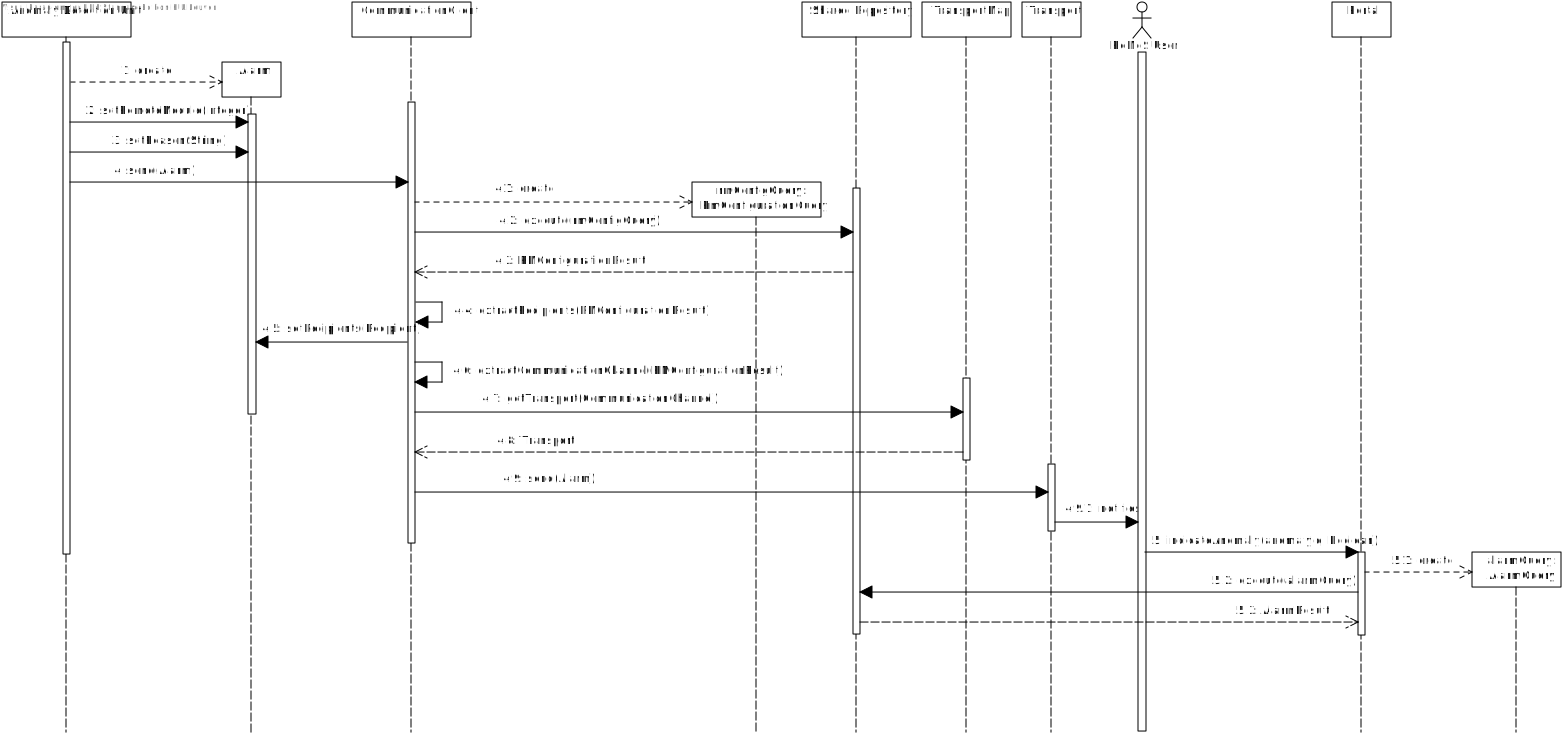
\includegraphics[width=\textwidth]{figs/scenario-5-10.pdf}
		\caption{Sequence diagram for the ``Alarm data transmission: ReMeS'' scenario}
		\label{fig:scenario-5-10}
	\end{centering}
\end{figure}

\npar In step 4.1 a RemoteModuleConfigurationQuery is drafted. This is a read
query to retrieve the configuration of the remote module (which is contained in
the Alarm). This configuration contains the alarm recipients and the
communication channel.

\npar In step 5 a ``notifies'' message is drawn to indicate that the ReMeS user
is physically contacted.

\npar In step 5.1 a store query is constructed. This query contains whether or
not the detected anomaly was correct. The returned result (AlarmResult) is empty
since it is a store query.

